\chapter{Planificación}

Antes de hablar de detalles de implementación, tenemos que pensar en la metodología y el control de calidad de la solución a construir.

\section{Metodología}

Necesito una metodología \textbf{que ponga al usuario en el centro} y permita una \textbf{retroalimentación rápida.} \\
\textbf{La metodología ágil} evita la documentación intensiva de requisitos y más diagramas de los necesarios, en favor de la iteración y la adaptación a requisitos cambiantes.\\

Otro principio de esta filosofía son las aportaciones frecuentes de código que aporten valor al usuario. Para esto,
necesitamos organizar la funcionalidad en bloques y asegurarnos de que los cambios en el código siempre surgen
de una necesidad del usuario. \\ \\
Las iniciativas, épicas e historias de usuario ayudan a esa organización.
Además, es importante que \textbf{los commits referencien a estas tareas,} así podemos
saber no solo quién ha escrito una línea de código sino también \textbf{por qué}, que siempre deberá responderse con una historia de usuario (\ref{subsec:hu}) o un issue (\ref{subsec:issue}).

\begin{figure}[H]
\centering	
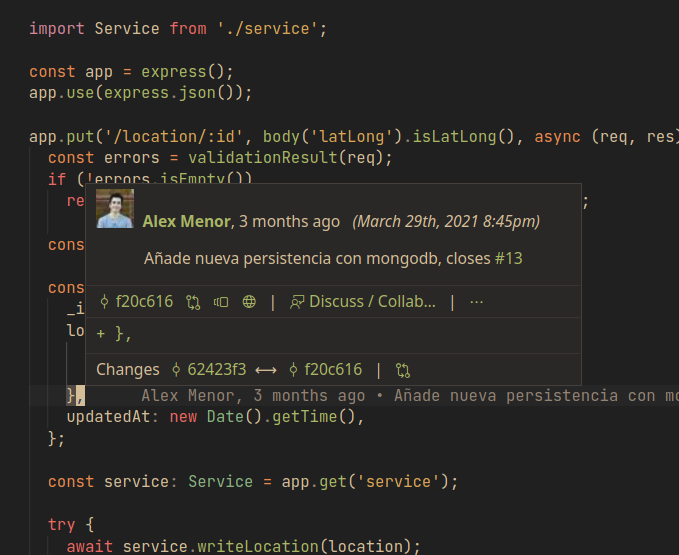
\includegraphics[scale=0.6]{git.png}
\end{figure}

Además, aplicando técnicas de design thinking, se ha hecho un análisis de "Personas" \cite{personas}. Ver anexo \ref{anexo}.

\subsection{Control de versiones}
Como sistema de control de versiones utilizo Git y como repositorio remoto GitHub \cite{repo}. Además, como veremos en la sección \ref{sec:inc} y \ref{sec:cal} GitHub
también nos permite implementar los flujos de integración continua y organizar las tareas.

\subsection{Iniciativas}\label{sec:inc}
\textbf{Son grandes grupos de funcionalidad, independientes entre sí, que sirven para atacar el problema.}
Acorde a lo explicado en la sección \ref{sec:obj}, he propuesto las tres iniciativas y las he 
reflejado como proyectos dentro del repositorio de GitHub.
\begin{figure}[H]
\centering	
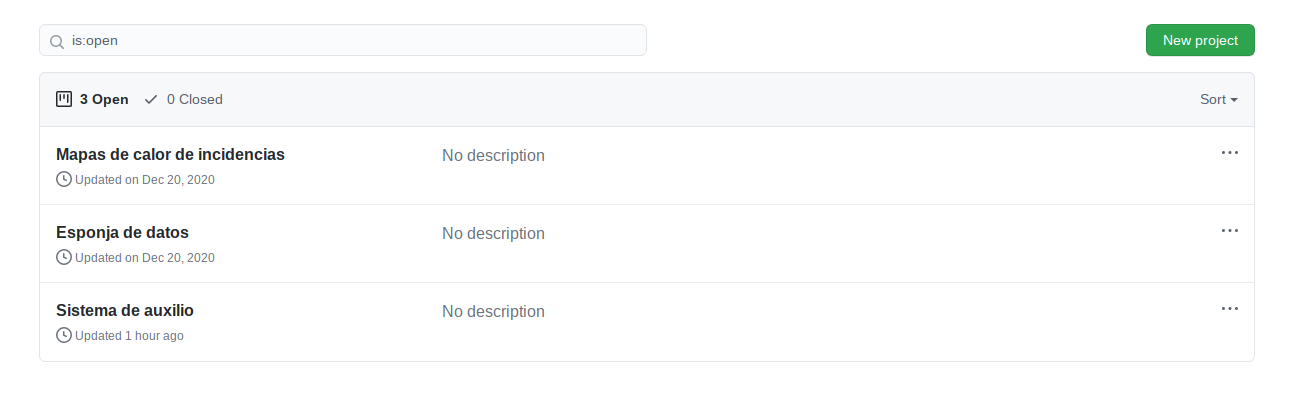
\includegraphics[scale=0.4]{iniciativas.png}
\end{figure}

\subsection{Épica}
Una iniciativa está formada por varias épicas. \textbf{Una épica por si sola no es una solución al problema}, pero todas las épicas de una iniciativa contribuyen a la solución.
Por ejemplo, para la iniciativa del sistema de auxilio, tenemos 
como épicas el frontend y el backend. Se reflejan en GitHub como milestones.
\begin{figure}[H]
	\centering
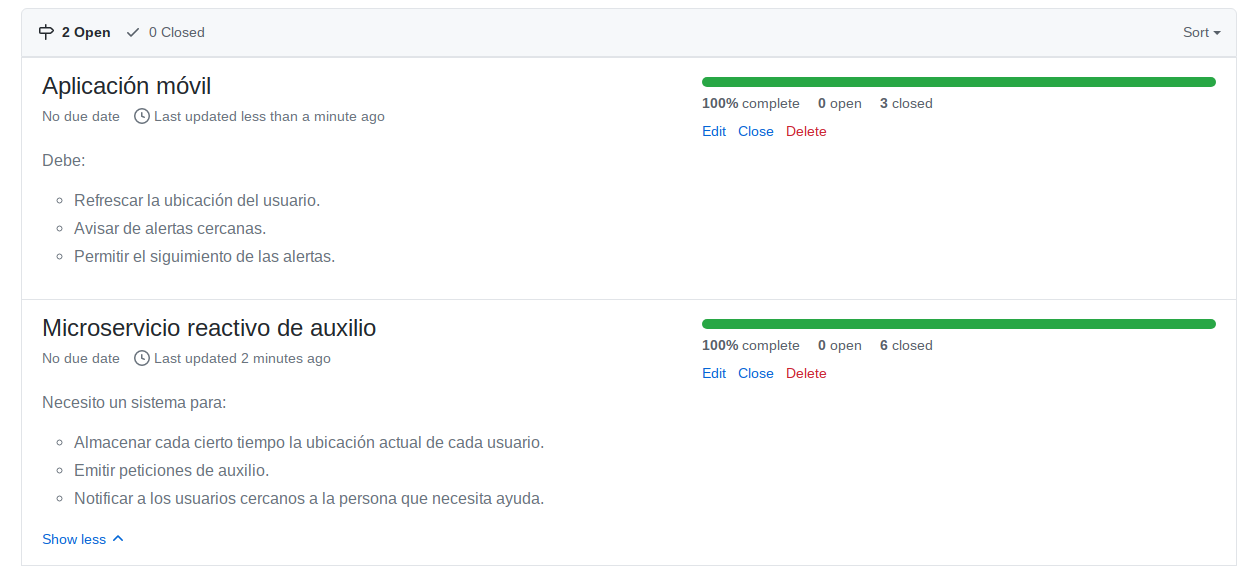
\includegraphics[scale=0.4]{milestones.png}
\end{figure}


\subsection{Historia de usuario}\label{subsec:hu}
Una épica a su vez está formada por varias historias de usuario que definen \textbf{una funcionalidad que el usuario espera en una solución}, de la forma:\\ \textit{Como [rol] quiero [funcionalidad] para [razón].}\\

A la hora de implementar una historia de usuario, esta se puede definir con requisitos más detallados.

\begin{figure}[H]
	\centering	
	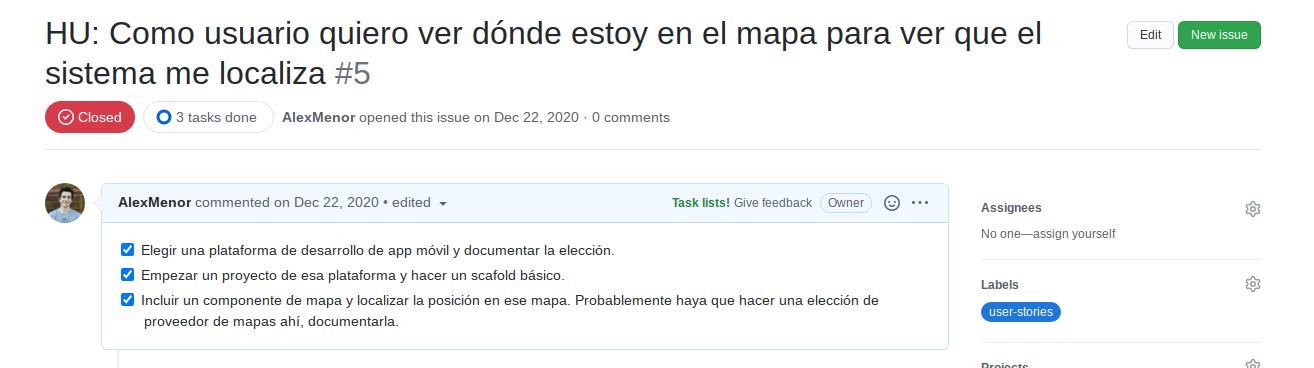
\includegraphics[scale=0.4]{hu.png}
	\end{figure}

\subsection{Issues}\label{subsec:issue}
\textbf{Cuando no se obtiene el comportamiento esperado}, podemos abrir un issue que se cerrará con un commit que lo solucione e idealmente un test que lo detecte.

\begin{figure}[H]
	\centering	
	
\includegraphics[scale=0.4]{issue.png}
	\end{figure}

	También pueden ser issues tareas que faciliten el mantenimiento del código.

\begin{figure}[H]
	\centering	
	
\includegraphics[scale=0.4]{issue2.png}
	\end{figure}


\section{Control de calidad}\label{sec:cal}

Para asegurar la calidad del proyecto necesitamos utilizar \textbf{integración continua con tests y análisis estático del código} por medio de linters (ver sección \ref{sec:tools}).


Cada vez que se hace un commit, se ejecutan todos estos procesos automáticamente.

La presencia de tests, de la que hablo con más detalle en la sección \ref{sec:tests}, nos permite, entre otras cosas, refactorizar con más 
tranquilidad. \\

Para cubrir la parte de integración continua he utilizado Github Actions,  configurando en formato \textit{yaml} todos los flujos.\\
La implementación continua de los tests y linters dependen del lenguaje y otros detalles de implementación, por tanto
son distintos para cada entorno.
\begin{figure}[H]
	\centering	
	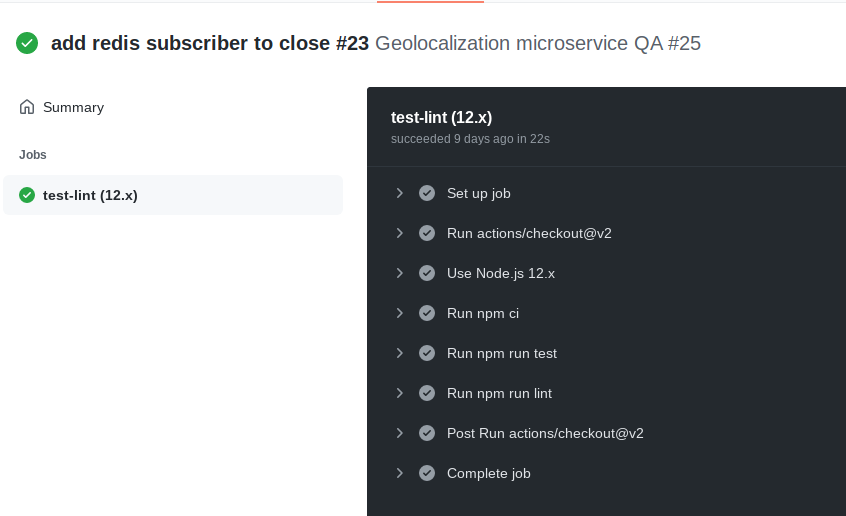
\includegraphics[scale=0.4]{ci.png}
	\end{figure}



